\documentclass[../main.tex]{subfiles}

\begin{document}

	Dentro del estudio de las reacciones de fusión en reactores, una parte importante se dedica al plasma que entrará en contacto con las superficies del tokamak. Si bien se menciono que, lo que se busca es confinar el plasma dentro del reactor para que no haya contacto con las paredes, es necesario eliminar impurezas del plasma, además de otras funciones importantes que se relevan a las superficies dentro del reactor. Por eso, es importante saber cómo se comportará el plasma en esas regiones. Una de las cosas a considerar es que, debido a la baja inercia y alta temperatura de los electrones, estos tienen un mayor flujo que los iones en la superficie de las paredes. Esto induce la formación de un potencial negativo flotante, que se ajusta hasta igualar los flujos de partículas cargadas en la pared. Este potencial de pared flotante es apantallado por el plasma, llegando a tener influencia hasta unas cuantas longitudes de Debye. Esta región se denomina funda o Sheath, y entre sus características, tenemos que la densidad de electrones es menor que la de los iones. El criterio de Bohm establece que, las partículas positivas (iones) acelerarán a través de un pequeño campo eléctrico ubicado en la frontera de la funda (Sheath edge) y que abandonaran la región del plasma cuasineutro, a velocidades del sonido en el plasma, dirigiéndose a las paredes.
	%----------------------------------------------
	
	\section{La SOL e Interacción Plasma-Pared}
	\lhead[\thepage]{\thesection. Interacción Plasma-Pared}
	%------------------------------------------
	
	Entre las funciones de la superficie del reactor, tenemos que las paredes de este deben minimizar la producción de polvo, que puede crear perturbaciones dentro (o en el borde) del plasma, y por lo tanto afectar el rendimiento de la fusión. Debe asegurar la integridad del vació producido dentro del reactor. También proporcionar el combustible que se utilizará para las reacciones de fusión. Finalmente, tiene que contribuir con el bombeo o eliminación, de las partículas generadas luego de la reacción, que después de haber transmitido su energía (cinética) a los iones circundantes, tendrán que ser removidos del plasma, como los restos de helio. Entonces, es importante definir la parte de la pared que entrará en contacto con el plasma, y se encargará de recibir a las partículas, cuya energía restante no ha sido eliminada por algún proceso disipativo. Para hacer esto, se pueden usar dos configuraciones distintas dentro de un reactor. Por un lado, tenemos el Limitor, que es una estructura metálica, cuya forma depende de cómo se lo ubique dentro del reactor, y cuya superficie tiene contacto con una región del plasma externo. Sabemos que dentro del tokamak, tenemos superficies de flujo magnético formadas por las líneas helicoidales de campo magnético. Se dice que una superficie es cerrada si ninguna línea de campo, que conforma la superficie, tiene contacto con alguna superficie sólida. Mientras que, una superficie abierta será aquella cuyas líneas de campo atraviesen alguna superficie sólida. Se tendrán, entonces, algunas superficies de flujo magnético que no tengan contacto con alguna parte material del reactor, mientras que algunas sí lo harán. A la última superficie cerrada se le denomina LCFS por sus siglas en ingles (Last closed flux surface). \\
    
        \begin{figure}[h]
        \centering
        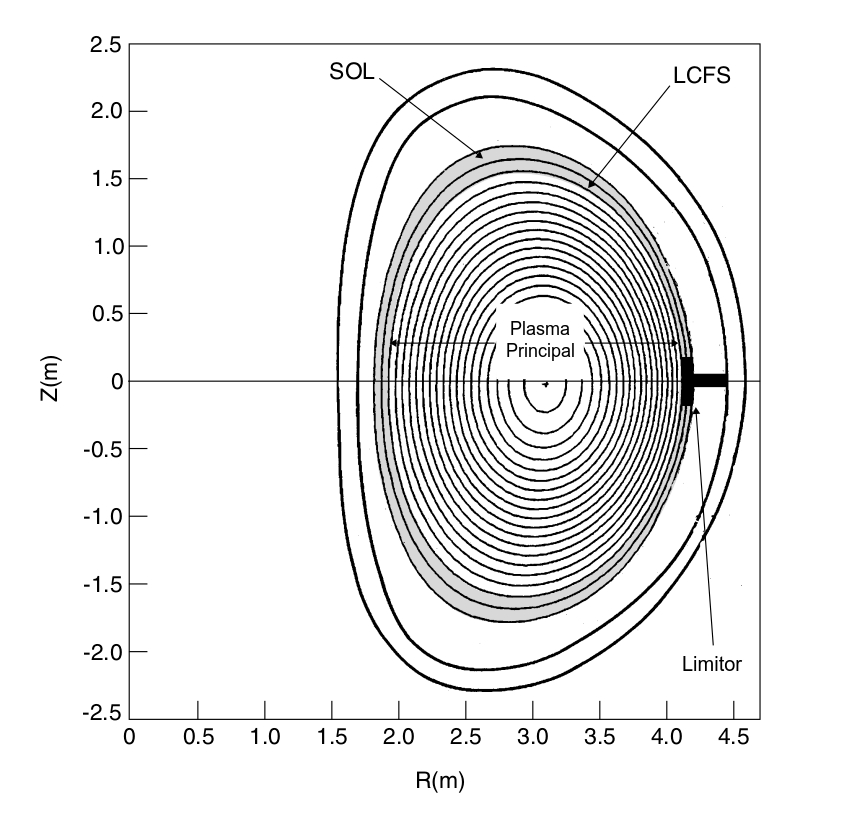
\includegraphics[width=0.7\textwidth]{Images/sol_lcfs.jpg}
        \caption{Sección transversal del reactor de fusión JET. Observamos el conjunto anidado de superficies de flujo magnético, y la última de estás denominada LCFS. La región del plasma en contacto con el limitor, es a lo que llamamos la SOL \cite{stangeby2000plasma}.}
        \label{fig:sol_jet}
        \end{figure}
    
    Más allá de la LCFS, nos encontramos con la parte del plasma denominada SOL por sus siglas en ingles (Srape-Off Layer). Está región del plasma es la que tendrá contacto directo con el mismo. Otra configuración, que permite que las líneas de campo magnético helicoidales tengan contacto con una superficie sólida, son los Divertores. Esta configuración se logra mediante el uso de ciertos imanes que, modifican el campo magnético poloidal y crean un punto nulo o punto X en cierta región del plasma. En este punto, las líneas magnéticas poloidales se separan, y terminan haciendo contacto con alguna superficie sólida del reactor. Consideremos ahora la SOL o capa de raspado, como se lo conoce también. Esta es la capa exterior del plasma que esta en contacto directo con las superficies designadas del reactor. Juega un papel importante, porque determina realmente, el efecto del plasma en la propia pared, y también influye en el comportamiento del núcleo del plasma, en algunas circunstancias. El espesor de la SOL resulta de un equilibrio entre la dinámica de campo cruzado y paralelo, y podemos estimarlo para un caso simple de configuración con un limitador, según la Figura \ref{fig:sol}. \\
    
    \begin{figure}[h]
        \centering
        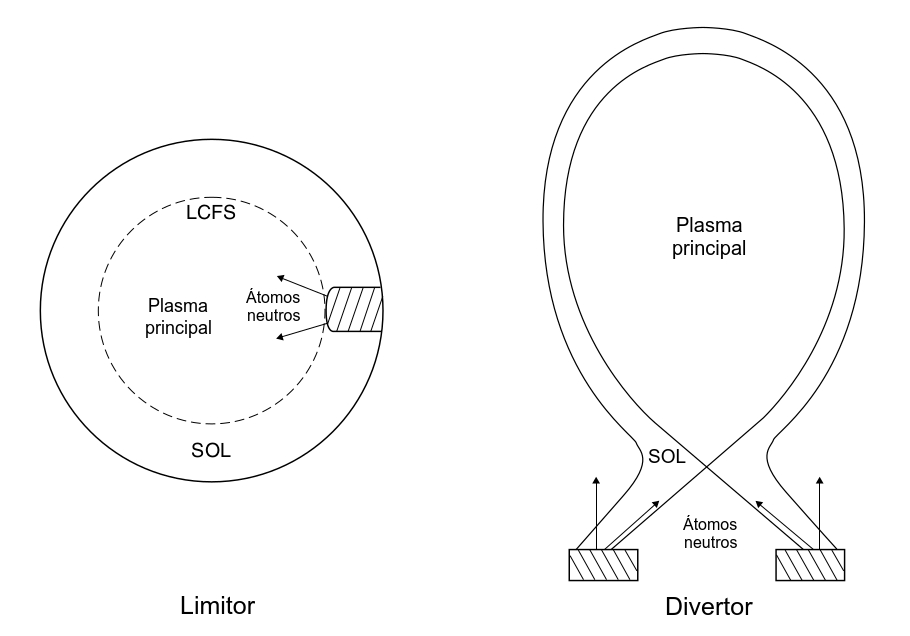
\includegraphics[width=0.7\textwidth]{Images/limitor_divertor.jpg}
        \caption{A la izquierda, tenemos la configuración tipo Limitor, en donde la región en contacto con el plasma, sobresale por una de las paredes. A la derecha, tenemos la configuración tipo 
        Divertor. Para este caso, se modifican las líneas magnéticas exteriores, para que el plasma en esa región se dirija a la parte inferior del tokamak. Estas superficies también actúan como fuentes de átomos neutros, debido a que las partículas cargadas se recombinan al llegar ahí \cite{stangeby2000plasma}.}
        \label{fig:lim_div}
        \end{figure}
    
    Las partículas tenderán a difundirse en cierto grado a las superficies externas del plasma, lo que se conoce también como dinámica de campo cruzado. Podemos calcular el flujo de partículas usando la ley de Fick $\Gamma_{\perp} = -D_{\perp} \partial n/\partial r$, donde el coeficiente de difusion $D_{\perp}$ es respecto de la dirección normal a las superficies magnéticas. Luego, establecemos un balance entre el número de partículas que ingresan a la SOL y el número de partículas que impactan en las superficies del limitor
    \begin{align}
         &\left|\Gamma_{\perp}\right|(2\pi r_0)(2\pi R_0) = 2nc_sL_{SOL}[2\pi(r_0 + R_0)].
    \end{align}
    La parte izquierda, es el número de partículas que ingresan a la SOL por segundo. Para esto se multiplico el flujo de partículas, por el área total de la superficie. Esta se puede calcular tomando la misma aproximación cilíndrica que en la Figura \ref{fig:superficie_magnetica}(b). La parte derecha es el número de partículas que golpean el limitor por segundo. El factor dos es debido a que se consideran la parte superior e inferior del limitor. Reemplazando $\Gamma_{\perp}$ tenemos que
    \begin{align}
         D_{\perp}\left|\frac{\partial n}{\partial r} \right|(2\pi r_0)(2\pi R_0) &= 2nc_sL_{SOL}[2\pi(r_0 + R_0)], \\
         \pi a R_0 D_{\perp} \frac{n}{L_{SOL}} &\approx nc_sL_{SOL}\left(R_0+r_0\right),
         \\
         L_{SOL} &\approx \sqrt{\frac{\pi aR_0D_{\perp}}{c_s\left(R_0+r_a\right)}},
    \end{align}
    donde $\left|\partial n/\partial r\right| \approx n/L_{SOL}$, es decir, se estima que la densidad varía en una escala de longitud igual a $L_{SOL}$. Entonces, para obtener un valor aproximado se tiene en cuenta que $D_{\perp}$ no coincide con valores clásicos típicos, por lo que se obtienen valores de manera experimental. Estos valores son del orden de $\mathrm{1 \ m^2 \ s^{-1}}$. La velocidad del sonido del plasma $c_s$, se obtiene mediante la siguiente expresión
    \begin{align}
        &c_s^2 = k_B \frac{T_e + T_i}{\left(m_e+m_i\right)}, \\
        &c_s \approx \left[k_B \frac{T_e + T_i}{\left(m_i\right)}\right]^{1/2}, \label{velocidad_sonido_plasma}
    \end{align}
    donde se despreció $m_e$ por ser pequeño en comparación. Para un plasma en equilibrio, $T_e = T_i = T$, y asumiendo una temperatura $T = 10^7 \ \mathrm{K}$, $r_0 = R_0/2 \approx 1.5 \ \mathrm{m}$ (valores aproximados), tenemos que  
    \begin{align}
        L_{SOL} \approx 0.3 \  cm.
    \end{align}
    Vemos que el grosor de la SOL es pequeña, del orden de $\mathrm{1 \ cm}$. Esto se puede explicar en función a la velocidad con la que las partículas ingresan a la SOL. Sea esta velocidad $v_\perp$, se puede estimar como \cite{stangeby2000plasma}
    \begin{align}
        v_{\perp} \approx \frac{D_{\perp}}{L_{SOL}}.
    \end{align}
    Además, se considera también una velocidad asociada a la dinámica de campo paralelo $v_\parallel$. Se entiende como la velocidad con la que las partículas se mueven a lo largo de la SOL, después de haber ingresado, y es del orden de $c_s$. Teniendo en cuenta los datos considerados
    \begin{align}
        v_{\perp} &\approx 10^2 \ ms^{-1}, \\
        v_{\parallel} \approx c_s &\approx 3\times10^5 \ ms^{-1}, \\
        &\frac{v_{\parallel}}{v_{\perp}}  \approx 3000
    \end{align}
    Entonces, vemos que para estas magnitudes consideradas (las cuales son típicas en un reactor de fusión), la velocidad con la que ingresan las partículas a la SOL, $v_\perp$, es mucho menor que la velocidad $v_\parallel$ con la que las partículas se aproximan al limitor. Estas se mueven muy rápido hacia las superficies de contacto, lo que provoca que el desplazamiento radial hacia afuera sea pequeño, y por lo tanto, $L_{SOL}$.

	\begin{figure}[hbtp]
        %\centering
        \subfigure[]{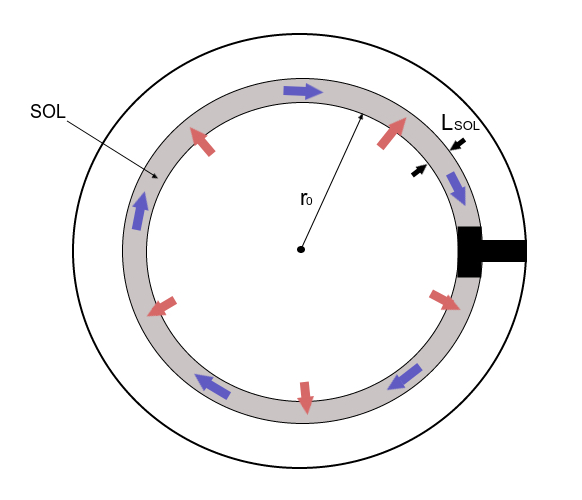
\includegraphics[width=8cm,height=7cm]{Images/sol_1.jpg}}
        \subfigure[]{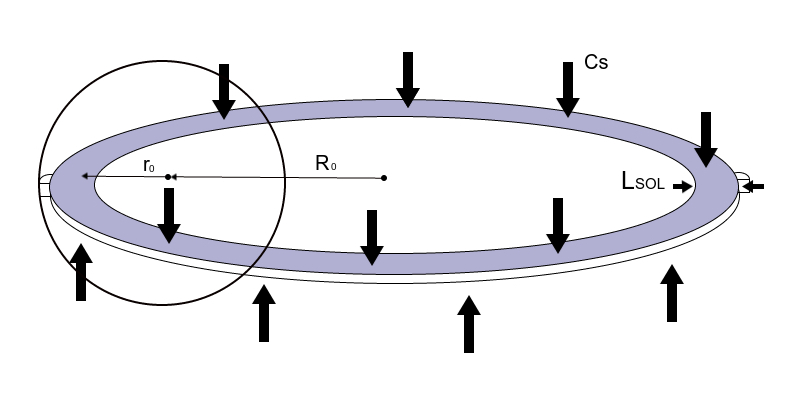
\includegraphics[width=8cm, height=5.5cm]{Images/sol_2.jpg}}
        \caption{a) Para un limitor en un modelo simplificado, podemos observar las dos dinámicas de campo descritas. Las flechas rojas describen el flujo de las partículas del plasma hacia la SOL, o dinámica de campo cruzado, debido a los efectos de difusión. Por otra lado, las flechas azules indican la dinámica de campo paralelo, lo que significa que las partículas salientes impactarán en la región asignada. b) Las partículas dentro de la SOL impactarán en la zona superior e inferior del limitor, debido a que ambas tienen contacto con el plasma. La velocidad a la que lo hacen, es igual a la velocidad del sonido del plasma $c_s$  .} \label{fig:sol}
    \end{figure}
	
   
	
%	Un flujo se produce, básicamente, por la presencia de %fuentes y sumideros para el líquido. En un plasma, %las paredes del reactor actúan como sumideros para %las partículas cargadas, las cuales se adhieren el %tiempo suficiente como para neutralizarse. Estos %átomos neutros pueden ser emitidos al plasma con %cierta energía térmica, pero también, ser %re-ionizados debido a los electrones energéticos. En %estado estacionario, se dice que el número de %recombinaciones de partículas cargadas es igual al %número de átomos neutros emitidos del plasma.\\
%
     %Ecuación de estado estacionario
%
%    Hay que tener en cuenta que las paredes actúan como %sumideros de carga eléctrica, más no de masa. Luego, %es necesario que una fuente externa dé energía para %poder ionizar las partículas neutras. Estas paredes %no solo sirven como sumidero para iones positivos, %sino también como una fuente de partículas neutras %para realimentar el plasma. Las cargas positivas son %capturadas en las paredes del reactor, mientras se  %van recombinando. Las partículas neutras que no %escapen rápidamente de la pared, se acumulan en la %misma. Cuando se llegue a cierto punto de saturación, %las partículas regresan al plasma, estableciéndose un %estado estacionario entre lo que sale y entra en el %plasma.
%
	%------------------------------------------
	
	\section{Debye Sheath}
	\lhead[\thepage]{\thesection. Debye Sheath}

	El número de electrones que inciden sobre la pared, no es el mismo que el número de iones que también lo hacen. Se debe tener en cuenta que la inercia de los electrones, favorece mucho más que estos lleguen a las paredes en mayores cantidades. Para mostrar esto, calculamos el flujo de partículas incidentes sobre la superficie de la pared, para un plasma cuyas partículas siguen la distribución de Maxwell. La velocidad promedio $<v>_{\alpha}$ de las partículas $\alpha$ la obtenemos también por medio de la distribución mencionada
        \begin{align}
            &\Phi_{\alpha} = \frac{1}{4}n_{\alpha}<v>_{\alpha}, \\
            &\Phi_{\alpha} =  \frac{1}{4}n_{\alpha}\left( \frac{8}{\pi} \right)^{1/2} \left( \frac{kT_{\alpha}}{m_{\alpha}} \right)^{1/2}, \\
            &\Phi_{\alpha} = n_{\alpha} \left( \frac{kT_{\alpha}}{2\pi m_{\alpha}} \right)^{1/2}.
        \end{align}
    Podemos hacer una comparación del flujo incidente de electrones e iones sobre las paredes. Considerando que las densidades son iguales debido a la cuasineutralidad del plasma, el factor $T_e/m_e$ en $\Phi_e$, es mucho más grande que $T_i/m_i$ en $\Phi_i$, dado que que los electrones tienen una masa mucho menor que los iones, y las temperaturas alcanzadas son mayores. Suponiendo que serán partículas alfa ($\mathrm{^4He}$), las que se dirigen hacia las superficies de contacto después de las reacciones de fusión, y además, que ambas especies se encuentran en equilibrio térmico, tenemos que
        \begin{align}
          &\frac{\Phi_{e}}{\Phi_{i}} = \frac{n_{e}}{n_{i}} \left( \frac{T_{e}/m_{e}}{T_{i}/m_{i}} \right)^{1/2}, \\
          &\frac{\Phi_{e}}{\Phi_{i}} = \left(\frac{m_{i}}{m_{e}} \right)^{1/2}, \\
          &\frac{\Phi_{e}}{\Phi_{i}} \approx \left( \frac{6.642 \times 10^{-27}}{9.109 \times 10^{-31}} \right)^{1/2}, \\
          &\frac{\Phi_{e}}{\Phi_{i}} \approx 85.39.
        \end{align}
    Este resultado nos dice que, por cada ion o partícula alfa que incide en la superficie, aproximadamente 85 electrones también lo hacen. Esta mayor presencia de partículas negativas establece un potencial flotante en la pared. Este potencial, de signo negativo, hace que el flujo de electrones disminuya, mientras que el flujo de iones que inciden aumente. A un determinado valor de potencial, los flujos en la pared se igualarán y la corriente neta será igual a cero. Se establece entonces una región, en donde los iones aceleran a altas velocidades por el potencial en la pared. Así, se tiene que el plasma, más allá de esta región se encuentra completamente apantallado del campo eléctrico producido por la acumulación de cargas negativas. Esta región, denominada Sheath, o Debye Sheath, debido a que su extensión solo es de unas cuantas longitudes de onda de Debye, es diferente al plasma contenido en el seno del reactor. Ya no se puede hablar de una cuasineutralidad, pues se verá que está diferencia en las densidades de ambas especies, es producto de una condición impuesta en la velocidad de los iones.
	%-------------------------------------------
	
	\section{Condición de Bohm para $T_i = 0$}
	\lhead[\thepage]{\thesection. Condición de Bohm para $T_i = 0$}
	
	%--------------------------------------------
	Como ya se mencionó, los iones alcanzan velocidades características, antes de acercarse lo suficiente a las superficies del objeto que contiene el plasma. Estas velocidades, que se alcanzan debido al potencial generado por el acumulamiento de partículas cargadas en las superficies, están limitadas por un valor mínimo. Entonces, para estudiar la dinámica de los iones al ingresar a la sheath, vamos a considerar un modelo unidimensional simplificado de la región considerada, en donde tenemos que la temperatura de los iones en el dominio principal del plasma (plasma neutro) es cero. Además, se asume que todos los iones se producen en un mismo punto, a partir de los procesos de ionización que sufren los átomos neutros, que regresan de la pared al seno del plasma neutro. Por último, se desprecian las colisiones en la sheath. Dado que los iones se acelerarán debido a este potencial, se puede considerar que una parte del campo eléctrico generado, penetra dentro del plasma. Esta región no es considerada dentro de la sheath, dado que los iones se aceleran aquí, para que posteriormente ingresen con cierta velocidad hacia las paredes. Entonces, denotando esta región como la pre-sheath, o una región intermedia entre el plasma principal y la sheath (Figura \ref{fig:sheath_edge}), tenemos que la velocidad en la frontera de la pre-sheath y la sheath (sheath edge) es $v_{se}$. \\
	
	\begin{figure}[h]
        \centering
        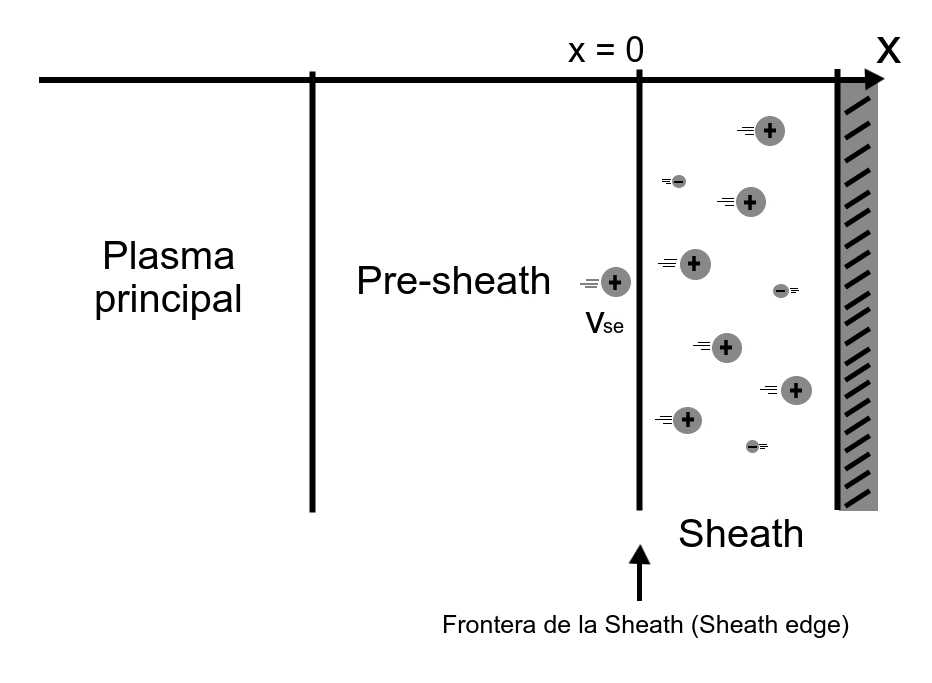
\includegraphics[width=0.7\textwidth]{Images/sheath_edge.jpg}
        \caption{Para estudiar la dinámica de los iones al ingresar a la sheath, el sistema se divide en tres regiones: El plasma principal, la pre-sheath, y la sheath.}
        \label{fig:sheath_edge}
        \end{figure}

    Con las consideraciones anteriores, planteamos la conservación de la energía entre la pre-sheath y la sheath. Dado que asumimos que los iones aceleran debido a la caída de potencial establecida en la pre-sheath, hasta una velocidad $v_{se}$, tenemos que dentro de la sheath 
    \begin{align}
        &\frac{1}{2} m_i v_i^2(x) = \frac{1}{2} m_i v_{se}^2 - e\phi(x), \label{presheath_sheath}\\
        & v_i(x) = \left(v_{se}^2 - \frac{2e\phi \left(x\right)}{m_i}\right)^{1/2}. \label{pot_sheath}
    \end{align}
    Tenemos en cuenta que, se toma de referencia un potencial $\phi=0$ en el dominio principal del plasma, por lo que los iones
    aceleran desde un potencial nulo, hasta un potencial negativo $\phi=\phi_{se}$ en la sheath edge, muy pequeño. El signo negativo en (\ref{presheath_sheath}) es
    debido a que la caída de potencial es negativa. Dado que asumimos, que los iones se producen muy por encima de la presheat, no tenemos fuentes de partículas en esta
    región, por lo que el flujo será constante, y se tendrá
    \begin{align}
        &\frac{d}{dx}\left( nv \right) = 0, \\
        &n_i(x)v_i(x) = n_0v_{se}. \label{equ_continuidad}
    \end{align}
    Combinando (\ref{pot_sheath}) y (\ref{equ_continuidad})

    \begin{align}
       & n_i(x) = n_0\left(1 - \frac{2e\phi \left(x\right)}{m_i}v_{se}^2\right)^{-1/2}. \label{densidad_sheath}
    \end{align}
    Para la densidad de electrones en esta región, consideramos que las velocidades de perdida no son muy grandes, debido a que los electrones se encuentran en un potencial repulsivo. Por lo tanto, la distribución de densidad es aproximadamente Maxwelliana, y dado que se encuentran además dentro de un potencial eléctrico, $\phi(x)$, usamos el factor de Boltzman, tal que
    \begin{align}
        n_e\left(x\right) = n_0exp\left(\frac{e\phi\left(x\right)}{k_BT_e}\right).
    \end{align}
    Ahora, dado que conocemos las densidades dentro de la sheath, calculamos el potencial eléctrico mediante la ecuación de Poisson
        \begin{align}
        \nabla^2 \phi &= -\frac{\rho}{\epsilon_0}, \\
        \epsilon_0 \frac{d^2\phi}{dx^2} &= e\left ( n_e\left(x\right) - n_i\left(x\right) \right), \\
        \epsilon_0 \frac{d^2\phi}{dx^2} &=  en_0\left[exp\left( \frac{e\phi\left(x\right)}{kT_e} \right) - \left(1 -\frac{2e\phi\left(x\right)}{m_i}v_{se}^2 \right)^{-1/2} \right], \label{poisson_dens}
        \end{align}
    y mediante el siguiente cambio de variables, resolvemos (\ref{poisson_dens})
    \begin{align}
        \chi \equiv -\frac{e\phi}{k_BT_e}, \ \xi &\equiv \frac{x}{\lambda_D}, \ M = \frac{v_{se}}{\left( kT_e/m_i \right)^{1/2}}, \\
        \frac{d^2\phi}{dx^2} = \frac{d}{dx}\left( \frac{d\phi}{d\xi}\frac{d\xi}{dx} \right) &= \frac{d}{dx}\left( \frac{-k_BT_e}{\lambda_De}\frac{d\chi}{d\xi} \right) = -\frac{k_BT_e}{\lambda_D^2e} \frac{d^2\chi}{d\xi^2}, \\
        -\epsilon_0 \frac{k_BT_e}{\lambda_D^2e}\frac{d^2\chi}{d\xi^2} &= en_0 \left[ exp\left(-\chi \right) - \left( 1 + \frac{2\chi}{M^2} \right)^{-1/2} \right], \\
        \frac{d^2\chi}{d\xi^2} &= \left( 1+\frac{2\chi}{M^2} \right)^{-1/2} - exp\left( -\chi \right), \label{final_equ}
    \end{align}
    donde $\lambda_D^2 = \epsilon_0kT_e/n_0e^2$. La ecuación (\ref{final_equ}) es no lineal, y corresponde al potencial eléctrico dentro de la sheath. Si multiplicamos esta expresión por $\chi\prime$ e integramos sobre una variable $\xi\prime$, donde se cumple que
    $d\chi = \chi\prime d\xi\prime$, resolviendo tenemos
    \begin{align}
        \int_0^{\xi}\chi\prime\chi\prime\prime d\xi\prime &= \int_0^{\xi} \left(1+\frac{2\chi}{M^2}\right)^{-1/2}\chi\prime d\xi\prime - \int_0^{\xi}e^{-\chi}\chi\prime d\xi\prime, \\
        \int_0^{\xi}\chi\prime\prime d\chi &= \int_0^{\xi} \left(1+\frac{2\chi}{M^2}\right)^{-1/2} d\chi - \int_0^{\xi}e^{-\chi} d\chi, \\
        \int_0^{\xi}d(\chi\prime) &= \int_0^{\xi} d\left(M^2\left[1+\frac{2\chi}{M^2}\right]^{1/2}\right)  + \int_0^{\xi}d\left(e^{-\chi}\right), \\
        \frac{1}{2}\left(\chi\prime^2-\chi\prime^2\left(0\right)\right) &= M^2\left[\left(1+\frac{2\chi}{M^2}\right)^{1/2} - 1\right] + e^{-\chi} - 1,
        \end{align}
    donde podemos asumir aproximadamente que el potencial, y el campo eléctrico en la sheath edge es cero. Entonces, tenemos que $\phi=E=0$ en $\xi=0$, y teniendo en cuenta que
    \begin{align}
        \chi\prime \equiv -\frac{e\phi\prime}{k_BT_e}, \\
        \chi\prime \equiv \frac{e}{k_BT_e}E,
    \end{align}
    se tiene $\chi\prime^2(0)=0$. Observamos entonces que la parte izquierda no es negativa, por lo que tomando la aproximación $\chi \ll 1$ o $-e\phi \ll k_BT_e$, y expandiendo la parte derecha en una serie de Taylor tenemos
    \begin{align}
        M^2\left(1+\frac{\chi}{M^2}-\frac{1}{2}\frac{\chi^2}{M^4}+...-1\right) &+ 1 - \chi + \frac{1}{2}\chi^2+...-1 \geq 0, \\
        \frac{1}{2}\chi^2\left(-\frac{1}{M^2}+1\right) &\geq 0, \\
        M^2 &\geq 1, \\
        v_{se} &\geq \left(\frac{k_BT_e}{mi}\right)^{1/2}, \\
       v_{se} &\geq c_s, \label{Bohm_condition}
    \end{align}
    \begin{figure}[h]
        \centering
        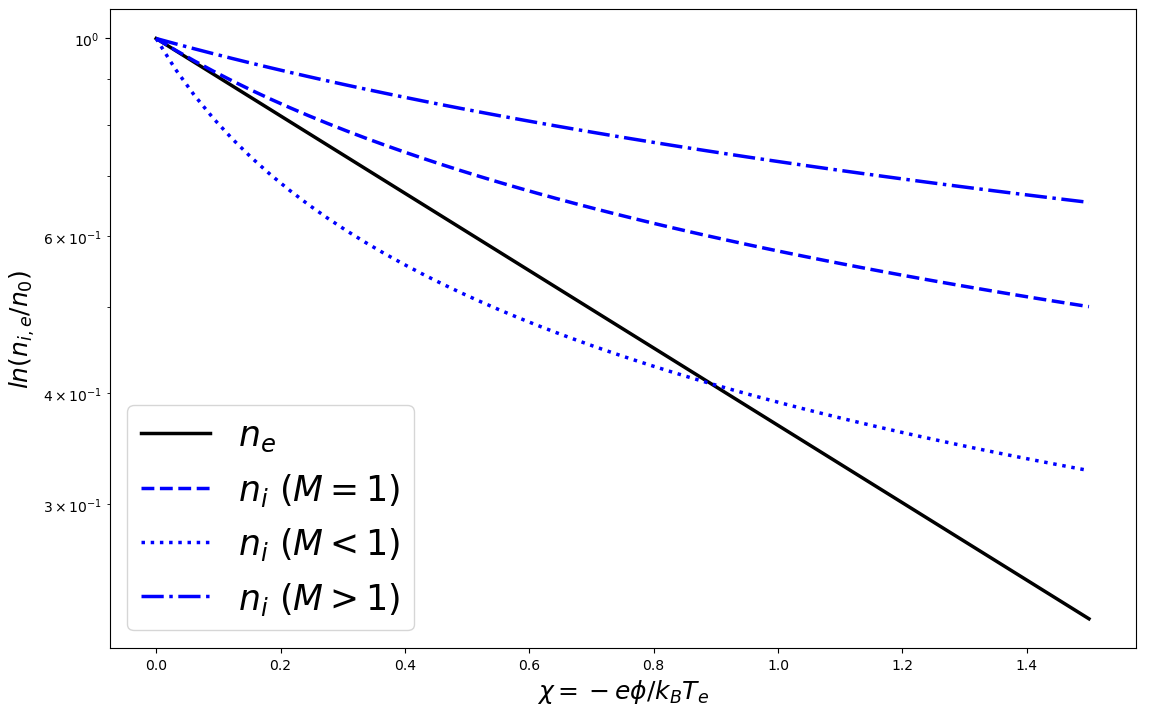
\includegraphics[width=0.9\textwidth]{Images/bohm_dens(1).png}
        \caption{Comportamiento de las densidades $n_e$ y $n_i$, según la condición de Bohm. Si los iones ingresan con una baja energía, entonces $n_i$ caería rápidamente, debido a que el campo en la sheath aumentaría la velocidad de los iones ($M<1$). En este caso $(n_e - n_i) >0$, lo que indicaría que el potencial se curva hacia arriba, en contradicción a la condición de Bohm. Por el contrario, si los iones ingresan con una alta energía, entonces $n_i$ caería más lento que $n_e$, lo que contrasta con la condición ($M\geq1$).}
        \label{fig:grafica_M}
        \end{figure}
        
    donde $c_s = \left( kT_e/m_i \right)^2$, es la velocidad del sonido en el plasma con $T_i=0$. La ecuación (\ref{Bohm_condition}) es conocida como
    la condición de Bohm. Hay que tener en cuenta ciertas cosas durante el análisis del proceso.
    Se sabe que, debido a la baja inercia de los electrones, podemos despreciar su energía cinética. Además, se establecerá un equilibro aproximado entre la fuerza ejercida por el campo eléctrico y el gradiente de 
    presiones, lo que evita que aceleren a velocidades muy altas y que aparezcan corrientes. Este equilibrio aproximado permite usar el factor de Boltzman para caracterizar la distribución de partículas.  Para los iones, la fuerza resultante será la suma del campo eléctrico y el gradiente de presiones, a diferencia de los electrones, que sufren un retardo debido al campo. La fuerza neta sobre el plasma es debida al gradiente de presiones total, dado que el plasma es aproximadamente neutro en el dominio principal.  Como ya hemos visto, existe un pequeño campo eléctrico, que penetra dentro del dominio principal del plasma, por lo que el apantalla miento no es perfecto. Este pequeño campo genera está asociado a una pequeña caída de potencial $\phi_{se$, que se encarga de que los iones aceleren, y mediante un cálculo \cite{stangeby2000plasma} se puede estimar que
              \begin{align}
                  \phi_{se} \approx  -0.7\frac{kT_e}{e}.
               \end{align}
    \begin{figure}[h]
        \centering
        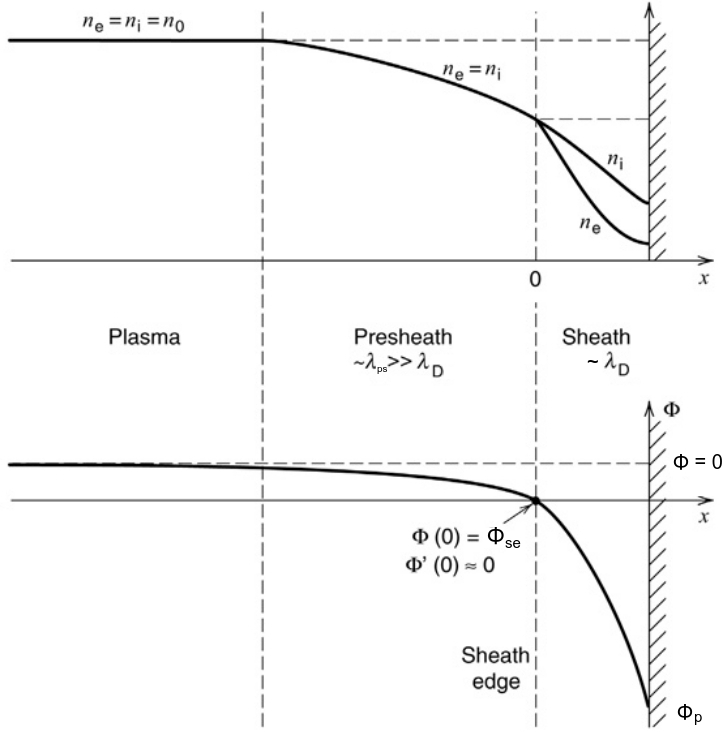
\includegraphics[width=0.7\textwidth]{Images/grafica_bohm_curvas.jpg}
        \caption{Variación espacial de las densidades $n_e$, $n_i$, y el potencial $\phi$. El plasma se mantiene neutro lejos de la pared, por lo que el potencial aquí será igual a cero. Sin embargo, en una región adyacente, se tendrá una pequeña caída $\phi_{se}$, por lo que los iones acelerarán hacia la pared. El gradiente de presiones hace los mismo respecto a los electrones, dado que el potencial tiene un efecto contrario para ellos. En una región de unas cuantas longitudes de Debye (sheath), el desbalance en la densidades de carga predominará, debido a que los iones ingresan a esta zona con velocidades por encima de la velocidad del sonido del plasma \cite{lieberman2005principles}.}
        \label{fig:potencial_dens_sheath_presheath}
        \end{figure}
	%--------------------------------------------
	\section{Condición de Bohm para $T_i \neq 0$}
	\lhead[\thepage]{\thesection. Condición de Bohm para $T_i \neq 0$}
    %---------------------------------------------
    Si consideramos que los iones se encuentran a cierta temperatura $T$ diferente de cero, podremos hablar ahora de una distribución de velocidades para los mismos, en la región anterior a la sheath (plasma principal y pre-sheath). El análisis previo nos permitió deducir la velocidad $v_{se}$ con la que los iones ingresan a la sheath. Sin embargo, este análisis se hizo teniendo en cuenta ciertas consideraciones. Sabemos que dentro de la sheath se tendrá una caída en la densidad de electrones, debido al potencial generado en la pared, que disminuye el flujo de estos hacia ella.
    También se tendrá una caída en la densidad de iones, pero está depende de cuan energéticos sean los iones
    al entrar a la sheath. Si los iones son muy energéticos, la caída de la densidad será lenta al inicio, pues el potencial no modificará demasiado la velocidad iónica. Por otra parte, si los iones no son muy energéticos, el potencial modificará las velocidades en mayor medida, por lo que la caída inicial de la densidad será mayor, e incluso, caer más rápido que la densidad de electrones, como lo muestra la Figura (\ref{fig:grafica_M}) para $M<1$. Entonces, cerca de la sheat edge
    \begin{align}
        \frac{d^2\phi}{dx^2} = e \frac{n_e - n_i}{\epsilon_0} > 0,
     \end{align}   
    lo que implica que el potencial $\phi$ tendría una curvatura hacia arriba, y contradice el hecho de que el potencial repele a los electrones al presentar una caída en la cercanía de la sheat edge.  En base a esto, podemos derivar una forma alternativa de la condición de Bohm, que nos permitirá trabajar con las distribuciones de velocidad para los iones \cite{baalrud2011kinetic}. Por lo tanto, si realizamos una expansión de la ecuación de Poisson alrededor de $\phi = 0$ tenemos que 
    \begin{align}
        \frac{d^2\phi}{dx^2} &= -\frac{\rho\left(\phi\right)}{\epsilon_0}, \\
        \frac{d^2\phi}{dx^2} &= -\frac{1}{\epsilon_0}\left[\rho(\phi = 0) + \frac{d\rho}{d\phi}_{\phi = 0} \phi+ \frac{1}{2!}\frac{d^2\rho}{d\phi^2}_{\phi = 0} \phi^2 ...\right].
    \end{align}
    Dado que $\rho(\phi = 0) = 0$, pues se toma la condición de cuasineutralidad, y despreciando el término de segundo orden $\phi^2$ por ser muy pequeño (dado que se está trabajando en un entorno cercano a cero, en donde $\phi$ tiene valores muy pequeños), tomamos el segundo término de la
    expansión, multiplicando la expresión resultante por $d\phi/dx$ e integrando respecto de x, obteniendo
    \begin{align}
        \frac{d^2\phi}{dx^2} &= -\frac{1}{\epsilon_0}\frac{d\rho}{d\phi}_{\phi=0}\phi, \\
        \int \frac{d^2\phi}{dx^2}\frac{d\phi}{dx} dx &= -\frac{1}{\epsilon_0}\frac{d\rho}{d\phi}_{\phi=0}\int \phi \frac{d\phi}{dx}dx,
    \end{align}
    \begin{align}
        \int d\left[\left(\phi\prime \right)^2 \right] &=  -\frac{1}{\epsilon_0}\frac{d\rho}{d\phi}_{\phi=0}\int\phi d\left(\phi\right), \\ 
        \frac{\left( \phi\prime \right)^2}{2} &= -\frac{1}{2\epsilon_0}\frac{d\rho}{d\phi}_{\phi=0}\phi^2 + C, \\
        \frac{E^2}{2} &+ \frac{1}{2\epsilon_0}\frac{d\rho}{d\phi}_{\phi=0}\phi^2 = C. \label{equ_phi_c}
    \end{align}
    En la escala de la longitud de la sheath (que es del orden de la longitud de Debye $\lambda_D$), $\phi \rightarrow  0$ $(E \rightarrow0)$ cuando $x/\lambda_D \rightarrow \infty$. Entonces, tenemos que $C=0$. Además, tomando la densidad total de partículas en el plasma, y derivando respecto de $\phi$, llegamos a que
    \begin{align}
        &\rho = \sum_p q_pn_p, \\
        &\frac{d\rho}{d\phi} = \sum_p q_p \frac{dn_p}{d\phi}, \label{derivada_phi}
    \end{align}
    calculando también $dn_p/dx$, y reemplazando en (\ref{derivada_phi})
    \begin{align}
        &\frac{dn_p}{dx} = \frac{dn_p}{d\phi}\frac{d\phi}{dx} = -E\frac{dn_p}{d\phi}, \\
        &\frac{dn_p}{d\phi} = -E^{-1}\frac{dn_p}{dx}, \\
        &\frac{d\rho}{d\phi} = - \sum_p q_p E^{-1}\frac{dn_p}{dx}. \label{equ_sum_rho}
    \end{align}
    Por último, de (\ref{equ_phi_c}), tenemos que $d\rho/d\phi_{\phi = 0} = -\epsilon_0E^2/\phi^2$. Esto nos dice que $d\rho/d\phi_{\phi = 0} \leq 0$. Significa entonces que, en el punto donde el potencial $\phi$ es igual a cero, la derivada de la densidad total será no positiva, es decir que en general, la densidad total decrecerá. Podemos decir, de manera aproximada y suponiendo que la función de densidad total es una función continua, que en el entorno de $\phi=0$ se cumplirá
    \begin{align}
        &\frac{d\rho}{d\phi} \leq 0.
    \end{align}
    Reemplazando (\ref{equ_sum_rho}), y teniendo en cuenta que $-1/E$ es un cantidad negativa, dado que $E = - d\phi/dx$, y  $\phi$ decrece hacia la pared, tenemos que
    \begin{align}
        &\sum_p q_p \frac{dn_p}{dx} \geq 0, \\
        &\sum_p q_p \int_{-\infty}^{\infty}\frac{\partial f_p}{\partial x}d^3v \geq 0, \label{bohm_sheath}
    \end{align}
    donde se uso $n_p = \int f_p d^3v$. La ecuación (\ref{bohm_sheath}) se le conoce también como criterio de la sheath, dado que se tomó como punto de análisis, un entorno cercano a $\phi=0$. Para ver el efecto de las funciones de distribución $f_p$, que pueden tomar las partículas en el plasma cerca de la sheath edge, usamos la
    ecuación de Boltzman 
    \begin{align}
        \frac{\partial f_p}{\partial t} + \mathbf{v}\cdot\frac{\partial f_p}{\partial \mathbf{r}} +\frac{\mathbf{F}}{m_p} \cdot\frac{\partial f_p}{\partial \mathbf{v}} = C\left(f_p\right). \label{ecu_de_boltzman}
    \end{align}
    Para nuestro caso, usaremos la ecuación de Vlasov unidimensional estacionaria, que se obtiene de (\ref{ecu_de_boltzman}), teniendo en cuenta que las fuerzas dentro del sistema son eléctricas, y despreciando el término colisional $C\left(f_p\right)$. Eliminando la parte temporal, obtenemos
    \begin{align}
        v_x\frac{\partial f_p}{\partial x} + \frac{q_p}{m_p}E\frac{\partial f_p}{\partial v_x} = 0. \label{vlasov}
    \end{align}
    Para poder despejar $\partial f_p/\partial v_x$ de (\ref{vlasov}), es necesario tomar el ``momento" de $1/v_x$, y reemplazando en (\ref{bohm_sheath}), separando también los términos correspondientes para los electrones ($e$) e iones ($i$), y asumiendo cantidades de carga iguales, tenemos
    \begin{align}
        &\int^{\infty}_{-\infty}\frac{1}{v_x}\left(v_x\frac{\partial f_p}{\partial x}\right)dv_x + \int^{\infty}_{-\infty}\frac{1}{v_x}\left(\frac{q_p}{m_p}E\frac{\partial f_p}{\partial v_x}\right)dv_x = 0, \\
        &\int^{\infty}_{-\infty}\frac{\partial f_p}{\partial x}dv_x  = - \frac{q_p}{m_p}E\int^{\infty}_{-\infty}\left(\frac{1}{v_x}\frac{\partial f_p}{\partial v_x}\right)dv_x, \\
        &\sum_p \frac{1}{m_p} \int _{-\infty}^{\infty}\frac{1}{v_x}\frac{\partial f_p}{\partial v_x}dv_x \leq 0, \\
        &\frac{1}{m_i} \int_{-\infty}^{\infty} \frac{1}{v_x}\frac{\partial f_i}{\partial v_x}dv_x \leq  -\frac{1}{m_e} \int_{-\infty}^{\infty} \frac{1}{v_x}\frac{\partial f_e}{\partial v_x} dv_x, \label{equ_pre_final}
    \end{align}
    el cual podemos considerar como el criterio generalizado o cinético de Bohm. Bajo ciertas consideraciones, podemos realizar un paso más en (\ref{equ_pre_final}), integrando por partes para obtener una forma familiar del criterio generalizado de Bohm. Sin embargo, para distribuciones usualmente esperadas, no se satisface este paso. Entonces, suponiendo que el integrando de la parte izquierda, $v_x^{-1}\partial f_i / \partial v_x$, es una función continuamente diferenciable, tenemos que
    \begin{align}
        \int _{-\infty}^{\infty} \frac{1}{v_x}\frac{\partial f_i}{\partial v_x}dv_x &= \int_{-\infty}^{\infty}\frac{\partial }{\partial v_x} \left( \frac{f_i}{v_x} \right)dv_x + \int_{-\infty}^{\infty}\frac{f_i}{v_x^2}dv_x, \\
        \int _{-\infty}^{\infty} \frac{1}{v_x}\frac{\partial f_i}{\partial v_x}dv_x &= \left(\frac{f_i}{v_x}\right)^{v_x = \infty}_{v_x = -\infty} + \int_{-\infty}^{\infty}\frac{f_i}{v_x^2}dv_x, \\
        \int _{-\infty}^{\infty} \frac{1}{v_x}\frac{\partial f_i}{\partial v_x}dv_x &= \int_{-\infty}^{\infty}\frac{f_i}{v_x^2}dv_x,
    \end{align}
    donde $f_i/v_x \rightarrow 0$ cuando $v_x \rightarrow \pm \infty$. Reemplazando finalmente en (\ref{equ_pre_final})
    \begin{align}
        \frac{1}{m_i} \int_{-\infty}^{\infty} \frac{f_i}{v_x^2}dv_x &\leq  -\frac{1}{m_e} \int_{-\infty}^{\infty} \frac{1}{v_x}\frac{\partial f_e}{\partial v_x} dv_x. \label{ecuacion_final}
    \end{align}    
    Para ver cómo es que la ecuación (\ref{ecuacion_final}) es análoga a la condición de Bohm, usaremos un modelo simple de distribución de velocidades para los iones \cite{stangeby2000plasma}, mientras que para los electrones tendremos una distribución Maxwelliana. Estas distribuciones serán las correspondientes a la sheath edge, pues es este el límite de la sheath, en donde las partículas ingresarán a la velocidad del sonido del plasma. Entonces, tenemos que
    \begin{align}
        f_i\left(v_x\right) &= \left\{ \begin{array}{lcc}
             n_0\left(2c_i\right)^{-1} & si \ v_{se}-c_i \leq v_x \leq v_{se}+c_i \\
             \\ 0 &  para \ otros \ valores \ de \ v_x
             \end{array}
   \right. \label{modelo_distribucion_iones} \\
        f_e\left(v_x\right) &= n_0\left(\frac{m_e}{2\pi k_BT_e}\right)^{1/2}exp\left(-\frac{m_ev_x^2}{2k_BT_e}\right),
        \end{align}
   
        \begin{align}
        \frac{1}{m_i} \int_{-\infty}^{\infty} \frac{f_i}{v_x^2}dv_x 
        &\leq  -\frac{1}{m_e} \int_{-\infty}^{\infty} \frac{1}{v_x}\frac{\partial f_e}{\partial v_x} dv_x, \\
        \frac{1}{m_i} \int_{v_{se}-c_i}^{v_{se}+c_i} \frac{n_0}{2c_i}\frac{1}{v_x^2}dv_x &\leq \frac{n_0}{k_BT_e}\left(\frac{m_e}{2\pi k_BT_e}\right)^{1/2}\int_{-\infty}^{\infty} exp\left(-\frac{m_ev_x^2}{2k_BT_e}\right) dv_x, \\
        \frac{1}{m_i} \frac{n_0}{2c_i}\left(-\frac{1}{v_{se}+c_i}+\frac{1}{v_{se}-c_i}\right) &\leq \frac{n_0}{k_BT_e}\left(\frac{m_e}{2\pi k_BT_e}\right)^{1/2}\left(\frac{2\pi k_BT_e}{m_e}\right)^{1/2}, \\
        \frac{1}{m_i} \frac{n_0}{2c_i}\left(\frac{2c_i}{v_{se}^2-c_i^2}\right) &\leq \frac{n_0}{k_BT_e}, \\
        \frac{k_BT_e}{m_i}  &\leq v_{se}^2-c_i^2, \\
        \frac{k_BT_e}{m_i}  &\leq v_{se}^2-\frac{k_BT_i}{m_i}, \\
        v_{se} &\geq \left(\frac{k_BT_e}{m_i} + \frac{k_BT_i}{m_i}\right)^{1/2}, \label{expresion_final_de_bohm}
    \end{align}
  
  donde se utilizado el valor característico $c_i = \left(k_BT_i/m_i\right)$. La expresión (\ref{expresion_final_de_bohm}) ya fue utilizada en (\ref{velocidad_sonido_plasma}), para el caso de un plasma en equilibrio térmico total, a una temperatura $T$. También podemos encontrar la condición de Bohm para el caso de $T_i = 0$, asumiendo ahora una distribución de velocidades unidimensional de la forma
    \begin{align}
        &f_i(v) = n_0\delta\left(v - v_{se} \right),
    \end{align}
   ya que uno de los supuestos en la derivación previa de la condición para $T_i=0$, era que todos los iones se originaban en un solo lugar por encima de la sheath edge, por lo que una función  de Dirac nos permite modelar esto. Reemplazando también en (\ref{ecuacion_final}) tenemos
   \begin{align}
       \frac{1}{m_i} \int_{\infty}^{-\infty} \frac{n_0}{v_x^2}\delta\left(v_x-v_{se}\right)dv_x 
        &\leq  \frac{n_0}{k_BT_e}, \\
        \frac{n_0}{m_iv_{se}^2}
        &\leq  \frac{n_0}{k_BT_e}, \\
        v_{se} &\geq \sqrt{\frac{kT_e}{m_i}}.
   \end{align}
   
   Podemos analizar ciertas cosas del modelo usado para la distribución de iones en (\ref{modelo_distribucion_iones}). Se puede observar que no existen velocidades de retroceso por parte de los iones, lo cual es algo que debe esperarse debido a la acción del potencial. Por otro lado, no se tienen velocidades iguales a cero en la sheath edge, lo cual conllevaría a divergencias en la integral. Por último, la integral esta fuertemente ponderada por la zonas de baja velocidad, que como ya se explicó, de la Figura (\ref{fig:grafica_M}), es esta parte de la densidad de iones la que acelerará hacia la sheath para mantener la validez de la condición. \\
   
   Hay que tener en cuenta que, la desigualdad (\ref{ecuacion_final})
   es muy limitada como ya se ha mencionado, y tiene ciertas deficiencias. Primero, el término de colisión en (\ref{ecu_de_boltzman})  no puede ser despreciado al tratar de obtener una expresión para $\partial f_p/\partial x$. Esto esta relacionado con el hecho de calcular, como se menciono líneas arriba, el momento de $1/v_x$ de la ecuación de Vlasov, lo que lleva a que se produzcan divergencias en el cálculo, a menos que se cumplan otras condiciones adicionales \cite{baalrud2011kinetic}. Segundo, también se menciono que la integración por partes en (\ref{equ_pre_final}) solo se cumplía si la función en la integral de la izquierda era continuamente diferenciable. Sin embargo, los experimentos en laboratorios para calcular las distribuciones de velocidades de las partículas, muestran que estas generalmente no satisfacen este paso. Sin embargo, el análisis, aunque limitado debido a las simplificaciones hechas, nos muestra un resultado que sí es comprobado experimentalmente, y que sirve para poder tener un punto de referencia, y posteriormente, modelos más detallados que los ya existentes.


\end{document}
